\chapter{Objects of arrays}
\label{Deck}

\index{array!of cards}

In the previous chapter, we defined a class to represent cards and used an array of \java{Card} objects to represent a deck.

In this chapter, we take another step toward object-oriented programming by defining a class to represent a deck of cards.
And we present algorithms for shuffling and sorting arrays.

%While reading the following sections, we recommend that you create a {\tt Deck.java} file and paste in all the examples.
%You will need {\tt Card.java} from the previous chapter for it to compile.

%So many of the examples are non-idiomatic; that is, they are not good Java.
%This transitional form should help you learn, but don't write code like this.

The code for this chapter is in {\tt Card.java} and {\tt Deck.java}, which are in the directory {\tt ch13} in the repository for this book.
Instructions for downloading this code are on page~\pageref{code}.


\section{The Deck class}
\label{deck}

The main idea of this chapter is to create a \java{Deck} class that encapsulates an array of \java{Card}s.
The initial class definition looks like this:

\begin{code}
public class Deck {
    private Card[] cards;

    public Deck(int n) {
        this.cards = new Card[n];
    }
}
\end{code}

\index{constructor}
\index{state diagram}

The constructor initializes the instance variable with an array of \java{n} cards, but it doesn't create any card objects.
Figure~\ref{fig.deckobject} shows what a \java{Deck} looks like with no cards.

\begin{figure}[!ht]
\begin{center}
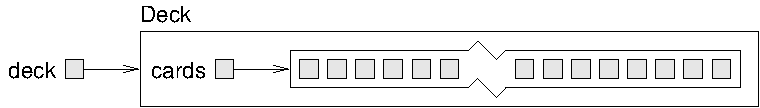
\includegraphics{figs/deckobject.pdf}
\caption{State diagram of an unpopulated \java{Deck} object.}
\label{fig.deckobject}
\end{center}
\end{figure}

We'll add a second constructor that makes a standard 52-card deck and populates it with \java{Card} objects:

\begin{code}
public Deck() {
    this.cards = new Card[52];
    int index = 0;
    for (int suit = 0; suit <= 3; suit++) {
        for (int rank = 1; rank <= 13; rank++) {
            this.cards[index] = new Card(rank, suit);
            index++;
        }
    }
}
\end{code}

This method is similar to the example in Section~\ref{cardarray}; we just turned it into a constructor.
We can now create a standard \java{Deck} like this:

\begin{code}
Deck deck = new Deck();
\end{code}

\index{printDeck}

Now that we have a \java{Deck} class, we have a logical place to put methods that pertain to decks.
Looking at the methods we have written so far, one obvious candidate is \java{printDeck} from Section~\ref{cardarray}.
%Here's how it looks, rewritten as an instance method of \java{Deck}:

\begin{code}
public void print() {
    for (int i = 0; i < this.cards.length; i++) {
        System.out.println(this.cards[i]);
    }
}
\end{code}

When you transform a static method into an instance method, it usually gets shorter.
We can simply type \java{deck.print()} to invoke the instance method.


\section{Shuffling decks}
\label{shuffle}

\index{shuffle}

For most card games you need to be able to shuffle the deck; that is, put the cards in a random order.
In Section~\ref{random} we saw how to generate random numbers, but it is not obvious how to use them to shuffle a deck.

One possibility is to model the way humans shuffle, which is usually dividing the deck in two halves and then choosing alternately from each one.
Since humans usually don't shuffle perfectly, after about seven iterations the order of the deck is pretty well randomized.

But a computer program would have the annoying property of doing a perfect shuffle every time, which is not very random.
In fact, after eight perfect shuffles, you would find the deck back in the order you started in!
(For more information, see \url{https://en.wikipedia.org/wiki/Faro_shuffle}.)

\index{pseudocode}

A better shuffling algorithm is to traverse the deck one card at a time, and at each iteration choose two cards and swap them.
Here is an outline of how this algorithm works.
To sketch the program, we will use a combination of Java statements and English.
This technique is sometimes called {\bf pseudocode}.

\begin{code}
for each index i {
    // choose a random number between i and length - 1
    // swap the ith card and the randomly-chosen card
}
\end{code}

\index{helper method}
\index{method!helper}

The nice thing about pseudocode is that it often makes clear what methods you are going to need.
In this case, we need a method that chooses a random integer between \java{low} and \java{high}, and a method that takes two indexes and swaps the cards at those positions.
Methods like these are called {\bf helper methods}, because they help you implement more complex algorithms.

\index{top-down development}
\index{program development}

And this process -- writing pseudocode first and then writing methods to make it work -- is called {\bf top-down development} (see \url{https://en.wikipedia.org/wiki/Top-down_and_bottom-up_design}).

\index{shuffle}

One of the exercises at the end of the chapter asks you to write the helper methods \java{randomInt} and \java{swapCards} and use them to implement \java{shuffle}.


\section{Selection sort}
\label{sorting}

\index{selection sort}
\index{sort!selection}

Now that we have messed up the deck, we need a way to put it back in order.
There is an algorithm for sorting that is ironically similar to the algorithm for shuffling.
It's called {\bf selection sort}, because it works by traversing the array repeatedly and selecting the lowest (or highest) remaining card each time.

During the first iteration, we find the lowest card and swap it with the card in the 0th position.
During the $i$th iteration, we find the lowest card to the right of $i$ and swap it with the $i$th card.
Here is pseudocode for selection sort:

\begin{code}
public void selectionSort() {
    for each index i {
        // find the lowest card at or to the right of i
        // swap the ith card and the lowest card found
    }
}
\end{code}

Again, the pseudocode helps with the design of the helper methods.
In this algorithm we can use \java{swapCards} again, so we only need a method to find the lowest card; we'll call it \java{indexLowest}.

One of the exercises at the end of the chapter asks you to write the helper method \java{indexLowest} and use it to implement \java{selectionSort}.


\section{Merge sort}
\label{mergesort}

\index{efficiency}

Selection sort is a simple algorithm, but it is not very efficient.
To sort $n$ items, it has to traverse the array $n-1$ times.
Each traversal takes an amount of time proportional to $n$.
The total time, therefore, is proportional to $n^2$.

\index{merge sort}
\index{sort!merge}

In the next two sections, we'll develop a more efficient algorithm called {\bf merge sort}.
To sort $n$ items, merge sort takes time proportional to $n \log_2 n$.
That may not seem impressive, but as $n$ gets big, the difference between $n^2$ and $n \log_2 n$ can be enormous.

For example, $\log_2$ of one million is around 20.
So if you had to sort a million numbers, selection sort would require one trillion steps; merge sort would require only 20 million.

The idea behind merge sort is this: if you have two subdecks, each of which has already been sorted, it is easy and fast to merge them into a single, sorted deck.
Try this out with a deck of cards:

\begin{enumerate}

\item Form two subdecks with about 10 cards each, and sort them so that when they are face up the lowest cards are on top.
Place both decks face up in front of you.

\item Compare the top card from each deck and choose the lower one.
Flip it over and add it to the merged deck.

\item Repeat step 2 until one of the decks is empty.
Then take the remaining cards and add them to the merged deck.

\end{enumerate}

The result should be a single sorted deck.
In the next few sections, we'll explain how to implement this algorithm in Java.


\section{Subdecks}

\index{subdeck}

The first step of merge sort is to split the deck into two subdecks, each with about half the cards.
So we might want a method, \java{subdeck}, that takes a deck and a range of indexes.
It returns a new deck that contains the specified subset of the cards:

\begin{code}
public Deck subdeck(int low, int high) {
    Deck sub = new Deck(high - low + 1);
    for (int i = 0; i < sub.cards.length; i++) {
        sub.cards[i] = this.cards[low + i];
    }
    return sub;
}
\end{code}

The first line creates an unpopulated subdeck.
Inside the \java{for} loop, the subdeck gets populated with copies of references from the deck.

\index{off-by-one}

The length of the subdeck is \java{high - low + 1}, because both the low card and the high card are included.
This sort of computation can be confusing, and forgetting the \java{+ 1} often leads to ``off-by-one'' errors.
Drawing a picture is usually the best way to avoid them.

\index{constructor}
\index{overload}

Figure~\ref{fig.subdeck} is a state diagram of a subdeck with \java{low = 0} and \java{high = 4}.
The result is a hand with five cards that are {\em shared} with the original deck; that is, they are aliased.

\begin{figure}[!ht]
\begin{center}
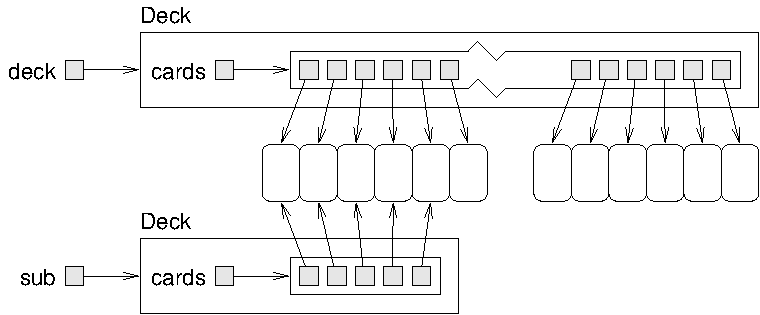
\includegraphics{figs/subdeck.pdf}
\caption{State diagram showing the effect of \java{subdeck}.}
\label{fig.subdeck}
\end{center}
\end{figure}

\index{aliasing}
\index{reference}

Aliasing might not be a good idea, because changes to shared cards would be reflected in multiple decks.
But since \java{Card} objects are immutable, this kind of aliasing is not a problem at all.


\section{Merging decks}

The next helper method we need is \java{merge}, which takes two sorted subdecks and returns a new deck containing all cards from both decks, in order.
Here's what the algorithm looks like in pseudocode, assuming the subdecks are named \java{d1} and \java{d2}:

\begin{code}
public static Deck merge(Deck d1, Deck d2) {
    // create a new deck big enough for all the cards

    // use the index i to keep track of where we are at in
    // the first deck, and the index j for the second deck
    int i = 0;
    int j = 0;
\end{code}

\begin{code}
    // the index k traverses the result deck
    for (int k = 0; k < result.cards.length; k++) {

        // if d1 is empty, d2 wins
        // if d2 is empty, d1 wins
        // otherwise, compare the two cards

        // add the winner to the new deck at position k
        // increment either i or j
    }
    // return the new deck
}
\end{code}

One of the exercises at the end of the chapter asks you to implement \java{merge}.


\section{Adding recursion}

Once your \java{merge} method is working correctly, you can try out a simple version of merge sort:

\begin{code}
public Deck almostMergeSort() {
    // divide the deck into two subdecks
    // sort the subdecks using selectionSort
    // merge the two halves and return the result
}
\end{code}

An exercise at the end of the chapter asks you to implement this algorithm.
Once you get it working, the real fun begins!
The magical thing about merge sort is that it is inherently recursive.

At the point where you sort the subdecks, why should you invoke the slower algorithm, \java{selectionSort}?
Why not invoke the spiffy new \java{mergeSort} you are in the process of writing?
Not only is that a good idea, it is {\em necessary} to achieve the $\log_2$ performance advantage.
\index{recursion}

To make \java{mergeSort} work recursively, you have to add a base case; otherwise it repeats forever.
A simple base case is a subdeck with 0 or 1 cards.
If \java{mergeSort} receives such a small subdeck, it can return it unmodified since it would already be sorted.

The recursive version of \java{mergeSort} should look something like this:

\begin{code}
public Deck mergeSort() {
    // if the deck is 0 or 1 cards, return it
    // divide the deck into two subdecks
    // sort the subdecks using mergeSort
    // merge the two halves and return the result
}
\end{code}

\index{leap of faith}

As usual, there are two ways to think about recursive programs: you can think through the entire flow of execution, or you can make the ``leap of faith'' (see Section~\ref{leap of faith}).
This example should encourage you to make the leap of faith.

When you used \java{selectionSort} to sort the subdecks, you didn't feel compelled to follow the flow of execution.
You just assumed it works because you had already debugged it.
And all you did to make \java{mergeSort} recursive was replace one sorting algorithm with another.
There is no reason to read the program any differently.

Well, almost.
You might have to give some thought to getting the base case right and making sure that you reach it eventually.
But other than that, writing the recursive version should be no problem.


\section{Vocabulary}

\begin{description}

\term{pseudocode}
A way of designing programs by writing rough drafts in a combination of English and Java.

\term{helper method}
Often a small method that does not do anything enormously useful by itself, but which helps another, more complex method.

\term{top-down development}
Breaking down a problem into sub-problems, and solving each sub-problem one at a time.

\term{selection sort}
A simple sorting algorithm that searches for the smallest or largest element $n$ times.

\term{merge sort}
A recursive sorting algorithm that divides an array into two parts, sorts each part (using merge sort), and merges the results.

%\term{insertion sort}
%Another sorting algorithm that inserts elements into place, one at a time.

\end{description}


\section{Exercises}

The code for this chapter is in the {\tt ch13} directory of {\tt ThinkJavaCode}.
See page~\pageref{code} for instructions on how to download the repository.
Before you start the exercises, we recommend that you compile and run the examples.


\begin{exercise}
You can learn more about the sorting algorithms in this chapter, and others, at \url{http://www.sorting-algorithms.com/}.
This site includes explanations of the algorithms, animations that show how they work, and analysis of their efficiency.
\end{exercise}


\begin{exercise}
The goal of this exercise is to implement the shuffling algorithm from this chapter.

\begin{enumerate}

\item In the repository for this book, you should find a file called {\tt Deck.java} that contains the code in this chapter.
Check that you can compile it in your environment.

\item Add a \java{Deck} method called \java{randomInt} that takes two integers, \java{low} and \java{high}, and returns a random integer between \java{low} and \java{high}, including both.
You can use the \java{nextInt} provided by \java{java.util.Random}, which we saw in Section~\ref{random}.
But you should avoid creating a \java{Random} object every time \java{randomInt} is invoked.

\item Write a method called \java{swapCards} that takes two indexes and swaps the cards at the given locations.

\item Write a method called \java{shuffle} that uses the algorithm in Section~\ref{shuffle}.

\end{enumerate}
\end{exercise}


\begin{exercise}
The goal of this exercise is to implement the sorting algorithms from this chapter.
Use the {\tt Deck.java} file from the previous exercise (or create a new one from scratch).

\begin{enumerate}

\item Write a method called \java{indexLowest} that uses the \java{compareCard} method to find the lowest card in a given range of the deck (from \java{lowIndex} to \java{highIndex}, including both).

\item Write a method called \java{selectionSort} that implements the selection sort algorithm in Section~\ref{sorting}.

\item Using the pseudocode in Section~\ref{mergesort}, write the method called \java{merge}.
The best way to test it is to build and shuffle a deck.
Then use \java{subdeck} to form two small subdecks, and use selection sort to sort them.
Then you can pass the two halves to \java{merge} to see if it works.
\index{testing}

\item Write the simple version of \java{mergeSort}, the one that divides the deck in half, uses \java{selectionSort} to sort the two halves, and uses \java{merge} to create a new, sorted deck.

\item Write a recursive version of \java{mergeSort}.
Remember that \java{selectionSort} is a modifier and \java{mergeSort} is a pure method, which means that they get invoked differently:

\begin{code}
deck.selectionSort();      // modifies an existing deck
deck = deck.mergeSort();   // replaces old deck with new
\end{code}

\end{enumerate}
\end{exercise}


\begin{exercise}
The goal of this exercise is to practice top-down programming by implementing ``insertion sort''.
Read about insertion sort at \url{http://www.sorting-algorithms.com/insertion-sort}.
Write a method named \java{insertionSort} that implements this algorithm.
\end{exercise}


\begin{exercise}
Write a \java{toString} method for the \java{Deck} class.
It should return a single string that represents the cards in the deck.
When it's printed, this string should display the same results as the \java{print} method in Section~\ref{deck}.

\index{StringBuilder}
\index{efficiency}

{\it Hint:} You can use the \java{+} operator to concatenate strings, but it is not very efficient.
Consider using \java{java.lang.StringBuilder}; you can find the documentation by doing a web search for ``Java StringBuilder''.
\end{exercise}
